\documentclass{article}
\usepackage[english]{babel}
\usepackage[utf8]{inputenc}
\usepackage[T1]{fontenc}
\usepackage{graphicx}
\usepackage{caption}
\usepackage{subcaption}
\usepackage{float}
\usepackage{wrapfig}
\usepackage{setspace}
\usepackage{cite}
\usepackage{url}
\usepackage{tikz}
\usetikzlibrary{positioning,trees}
\usepackage{soul}
\usepackage{color}
\definecolor{linkcol}{rgb}{0,0,0.4}
\definecolor{citecol}{rgb}{0.5,0,0}
\usepackage[pagebackref,hyperindex=true]{hyperref}
\hypersetup{colorlinks=true,linkcolor=linkcol,citecolor=citecol,urlcolor=linkcol}
\usepackage{xcolor}
\usepackage{listings}
%\lstset{
%	language=C++,
%	morekeywords={hsize_t},
%	keywordstyle=\color{blue},
%	commentstyle=\color{green},
%}

\lstdefinestyle{customc}{
  belowcaptionskip=1\baselineskip,
  breaklines=true,
  frame=L,
  xleftmargin=\parindent,
  language=C++,
  showstringspaces=false,
  basicstyle=\footnotesize\ttfamily,
  keywordstyle=\bfseries\color{blue!40!black},
  morekeywords={hsize_t},
  commentstyle=\itshape\color{purple!40!black},
  identifierstyle=\color{black},
  numberstyle=\color{red},
  stringstyle=\color{orange},
}

%\lstset{escapechar=@,style=customc}

\lstset{
language=C++,
basicstyle=\footnotesize\ttfamily,
keywordstyle=\bfseries\color{blue!60!black},
escapechar=@,
commentstyle=\itshape\color{purple!60!black},
numberstyle=\bfseries\color{red!60!black},
showstringspaces=false,
morekeywords={hsize_t},
breaklines=true,
literate=%
    {0}{{{\color{red}0}}}1
    {1}{{{\color{red}1}}}1
    {2}{{{\color{red}2}}}1
    {3}{{{\color{red}3}}}1
    {4}{{{\color{red}4}}}1
%    {5}{{{\color{red}5}}}1
    {6}{{{\color{red}6}}}1
    {7}{{{\color{red}7}}}1
    {8}{{{\color{red}8}}}1
    {9}{{{\color{red}9}}}1}


\begin{document}

\begin{titlepage}
\begin{center}
  \hfill
  \vspace{3.0cm}

  {\huge \textsc{IO Operations for wavepackets with HDF5 Interface in C++\\[10pt]
  }}
  ~\\[20pt]

  {\huge{Bachelor Thesis}}\\[2.5cm]

  {\emph{written by}}\\
  Florian Frei
  \\[0.6cm]
  {\emph{supervised by}}\\
  Dr. Vasile Gr\u{a}dinaru\\
  {\emph{and}}\\
  Prof. Dr. Ralf Hiptmair
  \\[2.5cm]

  Seminar for Applied Mathematics\\
  ETH Zurich
  \\[0.5cm]
  \emph{{Spring semester 2016}}
\end{center}
\end{titlepage}



\tableofcontents
\clearpage

\section{Introduction}
This thesis is about the continuation of the C++ implementation \cite{libwaveblocks} and allows a comparison to the Python implementation \cite{waveblocksnd}. The already existing framework is sufficient to generate simulations of different kind of Hagedorn wavepackets. The data produced is written in HDF5 binary format whereas the data from the C++ implementation is not easily comparable to the generated data from python. The writing process in the C++ implementation is currently done by using an extern project \cite{eigen3-hdf5}. The new implementation for writing binary HDF format in C++ will be explained in this thesis and also the new implementation allows easy comparison between Python and C++. It also incorporates a testing file which takes two HDF binary data files as arguments and compares the coinciding data. The testing file uses the well-known GoogleTest interface\cite{googletest}.

\section{HDF5 C++ Interface}
HDF stands for hierarchical data format which allows internal structure similar to a file system.
\subsection{Overview}
From the documentation we can conclude that the C++ interface is just a nice wrapper of the C interface. The corresponding classes and wrappers are shown in the table \ref{table:corrs}.\\
\begin{figure}[!h]
\centering
\begin{tabular}{|l|l|}
\hline
HDF5 C APIs&C++ Classes\\
\hline
Attribute Interface (H5A)&Attribute\\
Datasets Interface (H5D)&DataSet\\
Error Interface (H5E)&Exception\\
File Interface (H5F)&H5File\\
Group Interface(H5G)&Group\\
Identifier Interface (H5I)&IdComponent\\
Property List Interface (H5P)&PropList and subclasses\\
Dataspace Interface (H5S)&DataSpace\\
Datatype Interface (H5T)&DataType and subclasses\\
\hline
\end{tabular}
\caption{Table of correspondence between C and C++}
\label{table:corrs}
\end{figure}\\
The hierarchy of derivation of these classes is depicted in figure \ref{graph:hierarchy}.
\begin{figure}[h!]
\centering
\resizebox{\textwidth}{!}{
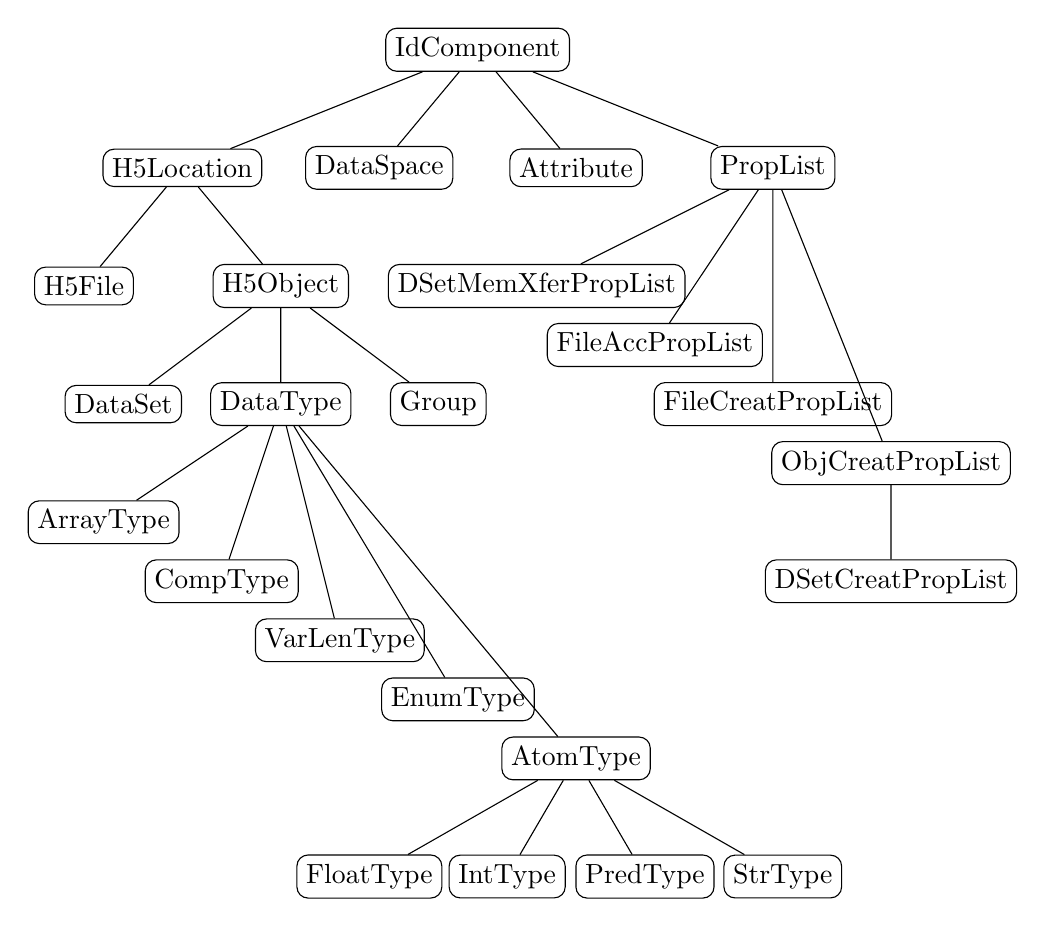
\begin{tikzpicture}[
baseline,
every node/.style = {shape=rectangle, rounded corners, draw, align=center},
]]
  \node {IdComponent}
    child[xshift=-1.5cm]
    {
        node{H5Location}
    	child[xshift=-0.5cm]{node{H5File}}
    	child[xshift=0.5cm]
    		{
    		node{H5Object}
    		child[xshift=-0.5cm]{node{DataSet}}
    		child{
    			node{DataType}
    			child[xshift=0.75cm]{node{ArrayType}}
    			child[xshift=0.75cm,yshift=-0.75cm]{node{CompType}}
    			child[xshift=0.75cm,yshift=-1.5cm]{node{VarLenType}}
    			child[xshift=0.75cm,yshift=-2.25cm]{node{EnumType}}
    			child[xshift=0.75cm,yshift=-3.0cm]
    				{
    				node{AtomType}
    				child[xshift=-0.375cm]{node{FloatType}}
    				child[xshift=-0.125cm]{node{IntType}}
    				child[xshift=0.125cm]{node{PredType}}
    				child[xshift=0.375cm]{node{StrType}} 
    				}
    			}
    		child[xshift=0.5cm]{node{Group}}
    		}
 	}
    child[xshift=-0.5cm]{node{DataSpace}}
    child[xshift=0.5cm]{node{Attribute}}
    child[xshift=1.5cm]{
    	node{PropList}
    	child[xshift=-0.75cm]{node{DSetMemXferPropList}}
    	child[xshift=-0.75cm,yshift=-0.75cm]{node{FileAccPropList}}
    	child[xshift=-0.75cm,yshift=-1.5cm]{node{FileCreatPropList}}
    	child[xshift=-0.75cm,yshift=-2.25cm]{
    		node{ObjCreatPropList}
    		child{node{DSetCreatPropList}}
    		}
    		};
\end{tikzpicture}
}
\caption{Depiction of derivation hierarchy}
\label{graph:hierarchy}
\end{figure}\\

%Throughout this thesis we will ignore the "H5" namespace and will always directly refer to the name of the object.\\
For our purposes we need to save a \textit{Hagedorn} wave packet in chosen time steps which consists of matrices and vectors. 
%overwork
For these we need a \textit{DataSpace} which allows us to write matrices and vectors in a time-dimension. In our case the time-dimension is arbitrarily chosen depending on the kind of the simulation. As such we need a \textit{DSetCreatePropList} which is used to describe properties such as chunk-dimension for matrices used in our case for time-dimension.\textit{Attributes} are used to save additional information such as the used time-step $\delta t$ in the simulation. For constructing a HDF5 binary file we need to use the \textit{File} class which simply uses a string argument as the filename. For neatness we want to have a intern structure for our data. For this we use the \textit{Group} class which is very similar to the file system and its folders for structuring. To write \textit{Eigen}-matrices we need the \textit{DataType} class which defines how to write these data types. Last but not least we need a \textit{DataSet} for every object we want to write to our binary file.

\subsection{Internally used types and states}
To work with the HDF5 library or an interface in general one needs to use the declared functions and types. Function arguments also have to be of an internal data type or class which the library expects at this position and sometimes these arguments also only have some valid states. All these are wrapped in a \texttt{namespace H5} which will be omitted thereafter. Therefore we will discuss in the next sections which objects and types are relevant for our purposes. For further information we refer to the official documentations \cite{hdf5cppdoc} \cite{hdf5cdoc}.
\subsubsection{hsize$\_$t}
Variables of this type represent native multiple-precision integer. This type is commonly used as an argument for library functions and substitutes mostly the internal \texttt{int} C++ type.
\subsubsection{H5std$\_$string}
\texttt{H5std\_string} is just an alias for the \texttt{std::string} type. This type is always used for naming library specific objects such as the name of a\textit{DataSet} or internal members of an \textit{DataType}.
\subsection{H5File}
A \textit{H5File} with default construction has already a \textit{Group} root "/". To construct a \textit{H5File}  a minimal number of two arguments are needed. Two additional optional arguments are the \textit{FileCreatPropList} and \textit{FileAccPropList} which allow further specification which is in our case not needed and the \texttt{H5P\_DEFAULT} is sufficient. First is the filename represented as a string as discussed before and the second argument defines the type of creation. There are just two possible values \textit{H5F\_ACC\_TRUNC} and \textit{H5F\_ACC\_EXCL} which are mutually exclusive. The former truncates the file and if it already exists erase all data previously stored in the file. The latter fails if the file already exists. We will work with \textit{H5F\_ACC\_TRUNC} because if the filename already exists means there is data for this simulation setup which will be overwritten which is not fatal because we can always repeat the simulation from before which results in the same data.
\subsection{Group}
We use \textit{Groups} to further structure our data in the file. Suppose we have a \textit{Hagedorn} wave packet and the corresponding energies with a time series then we would like to structure these in the file in a sub folder manner such as in figure \ref{graph:file}.

\begin{figure}[h!]
\centering
\resizebox{\textwidth}{!}{
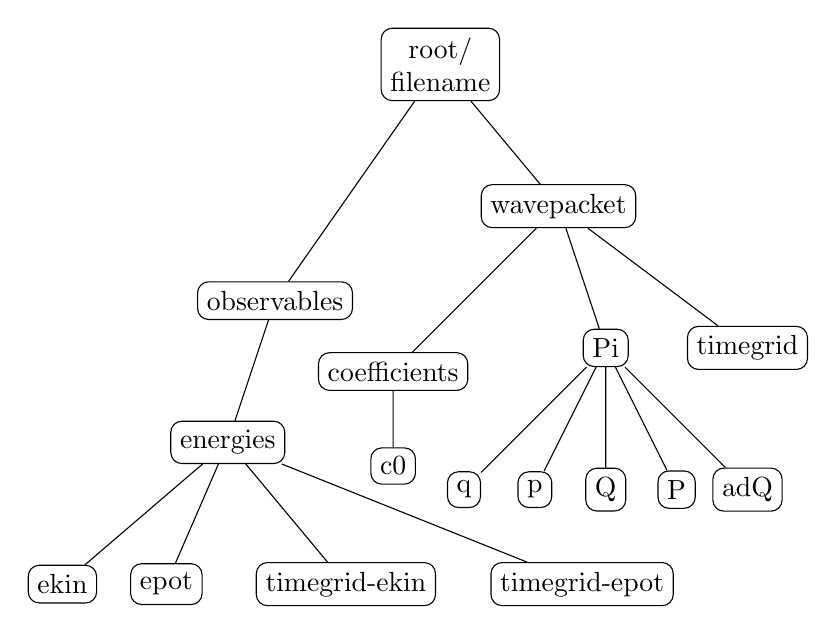
\begin{tikzpicture}[
baseline,
scale=1.2,
every node/.style = {shape=rectangle, rounded corners, draw, align=center},
]]
  \node {root/\\filename}
    child[yshift=-1cm,xshift=-1cm]
    {
    node{observables}
    child[xshift=-0.5cm]
            {
            node{energies}
    		child[xshift=0.5cm]{node{ekin}} 
    		child[xshift=0.1cm]{node{epot}}
    		child[xshift=0.5cm]{node{timegrid-ekin}}
    		child[xshift=1.5cm]{node{timegrid-epot}}
    		} 
    }
    child[xshift=0.5cm] 
    { 
    node {wavepacket}
    child[xshift=-0.25cm,yshift=-0.25cm]{node{coefficients}
    child[yshift=0.5cm]{node{c0}}}
    child[xshift=0.5cm]
    {
    node {Pi}
    child[xshift=1.5cm]{ node {q} }
    child[xshift=0.75cm] { node {p} }
    child { node {Q} }
    child[xshift=-0.75cm] { node {P} }
    child[xshift=-1.5cm] { node {adQ}}    
    }
    child[xshift=0.5cm]{node{timegrid}} 
	};
\end{tikzpicture}
}
\caption{Depiction of internal structure of a H5File}
\label{graph:file}
\end{figure}
This can be easily done when we use for every leaf of the graph in figure \ref{graph:file} a \textit{DataSet} and for every intermediate node a \textit{Group}. As already mentioned before a \textit{H5File} has root \textit{Group} "/" after creation. For implementing the structure in figure \ref{graph:file} one just needs to include the path in the name during creation. For example the name for the \texttt{coefficients} \textit{Group} we would use "/wavepacket/coefficents" as name and for \texttt{c0} \textit{DataSet} "/wavepacket/coefficents/c0".


\subsection{DataSet}
To allocate a \textit{DataSet} the HDF5-library needs four arguments. The order and types are \textit{string}, \textit{DataType}, \textit{DataSpace} and \textit{DSetCreatPropList}. All these will be explained in the following sections. The path as discussed above is the first argument. The type and dimension of the data are defined through the next two arguments. The last argument is property list at creation time to alter the layout of the data set. The \textit{DataSet} has three types of layouts to store raw data. These are \texttt{H5D\_COMPACT}, \texttt{H5D\_CONTIGUOUS} and \texttt{H5D\_CHUNKED}. The following graphic is meant to illustrate the inner workings of these layouts:

\begin{figure}[h!]
\centering
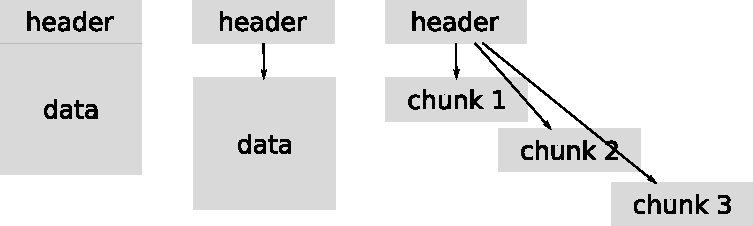
\includegraphics[width=\textwidth]{data_layout.pdf}
\caption{The three data layouts in \textit{DataSet}}
\label{fig:datalayout}
\end{figure}

If the data is not to large we can store it as \texttt{H5D\_COMPACT} meaning the data follows right after the header shown on the left. In case the data is larger but still somehow constant we use the \texttt{H5D\_CONTIGUOUS} layout in the middle meaning the header points to the data block which is stored contiguously in memory. The last case on the right is used if the size of the data is unknown. We store in the header the locations of all chunks meaning to add new data a new chunk will be appended in the header.

%A \textit{DataSet} is used as the location and representation for an object of interest. To construct a \textit{DataSet} we need four arguments. First argument is a string which represents the name and also the inner location in the file which will be explained later. The second argument describes the used \textit{DataType} to write data to this set. The third argument is a \textit{DataSpace} which describes the dimension of the \textit{DataSet}. The forth and last argument is a \textit{DSetCreatPropList} which describes inner properties of the DataSet for example the default fill value or the extensibility of the set.
\subsection{DataType}
For writing HDF format a \textit{DataType} object is needed as argument in the writing process. As shown in graph \ref{graph:hierarchy} \textit{DataType} is derived from an \textit{H5Object} and is further decomposed into various types for different usage. For writing floating point numbers for example the \textit{FloatType} is used. One could further change the characteristic of the default IEEE representation to other definitions if desired. It is obvious that for writing one uses \textit{IntType} for \texttt{int}, \textit{StrType} for \texttt{std::string}, \textit{PredType} for C++ intrinsic defined types such as \texttt{double}, \texttt{int}, \texttt{float} etc., \textit{ArrayType} for fixed sized arrays, \textit{VarLenType} for variable sized arrays, \textit{EnumType} for \texttt{enum}, and \textit{CompType} for simple compositions of atom types. In our case it is sufficient to use a \textit{CompType} default constructed because we will define our complex data type as a \texttt{struct} composed of two \texttt{doubles}.
%overwork
%The \textit{DataType} class describes how to write different kind of types and handles writing options. Every \textit{DataType} is given a name which is stored in a string used as its representation. As we can see from figure \ref{graph:hierarchy} \textit{DataType} is derived from \textit{H5Object} and is further decomposable in \textit{ArrayType}, \textit{AtomType}, \textit{CompType}, \textit{EnumType} and \textit{VarLenType}. For example when we want to write a native double and we don't care how it is represented on our system we would use a \textit{PredType} from \textit{AtomType} because it will use the definition from the operating system. When we would like to choose or define ourself how to write a double we would use the \textit{FloatType} from \textit{AtomType}. For cases where our data type is a struct of atomic types we would use the \textit{CompType}. For interested parties and further explanations we refer to the HDF5 official C++ documentation\cite{hdf5cppdoc} an C documentation \cite{hdf5cdoc}.
\subsection{DataSpace}
To describe the dimensionality of our data a \textit{DataSpace} object is needed. The construction of such a \textit{DataSpace} is straightforward. Firstly the library needs to know the number of dimensions. Secondly it has know the number of elements in each dimension. For the second argument we need to use an array of \texttt{hsize\_t} instead of an array of \texttt{int} because the library expects so. For example for a time grid \textit{DataSpace} the following code is sufficient:\\
%A simple way to construct such a \textit{DataSpace} is to call the constructor with two arguments. The first one is the \texttt{rank} of the space, which indicates the number of dimension the space will have. Following as the second argument is an \texttt{array} of type \texttt{hsize\_t} with dimensionality of length \texttt{rank}. In each entry is the number of elements we want in this dimension. 
\begin{lstlisting}
int rank = 1;
hsize_t size[rank];
size[0]=number_of_timesteps;
DataSpace limited_timespace(rank,size);
\end{lstlisting}
The problem herein lies in the number of time steps which is unknown when we construct our \textit{DataSpace}. This leads to another approach which is to define a unlimited \textit{DataSpace}. The library allows this if we add an additional argument in the creation. This argument is also an \texttt{array} of type \texttt{hsize\_t} and contains the maximum size of each dimension. This size has to be greater or equal than the used one previously as \texttt{size}. Here it is allowed to use the \texttt{H5S\_UNLIMITED} value in the array to indicate an unlimited \textit{DataSpace}.
\begin{lstlisting}
int rank = 1;
hsize_t size[rank] = {1};
hsize_t maxsize[rank]={H5S_UNLIMITED};
DataSpace unlimited_timespace(rank,size,maxsize);
\end{lstlisting}

\subsection{PropList}
This class is used to create a new property as an instance of some property class. These constructed default classes are: \texttt{H5P\_FILE\_CREATE} for \textit{H5FILE} creation, \texttt{H5P\_FILE\_ACCESS} for \textit{H5FILE} access, \texttt{H5P\_DATASET\_CREATE} for \textit{DataSet} creation, \texttt{H5P\_DATASET\_XFER} for raw data transfer and \texttt{H5P\_MOUNT} for \textit{H5File} mounting.


\subsection{DSetCreatePropList}
This property list is used to change the mentioned data layout in figure \ref{fig:datalayout}. %We use a \textit{DSetCreatPropList} to change the properties of how raw data is organized on disk and how the raw data is compressed. 
When default constructed a \textit{DataSet} is simple meaning \texttt{H5D\_COMPACT} but this doesn't allow us easy extension of the \textit{DataSet}. For allowing unlimited extension we change the property of how raw data is organized by creating this property list and changing the chunk dimension to the time step size.

\subsection{Attribute}
An \textit{Attribute} is used to write additional information to an existing \textit{Group} or \textit{DataSet} to describe the nature and/or the intended usage or the object. To create an \textit{Attribute} it has to be attached to an extisting \textit{Group} or \textit{DataSet}. The creation is similar to a \textit{DataSet} because the same arguments are needed except for the \textit{DSetCreatPropList} only the \texttt{H5P\_DEFAULT} is allowed.



\section{Eigen Interface}
For our purposes we need the storage format in \textit{Eigen/Core} for storing the subparts of the \textit{Hagedorn} wave packet. \textit{Eigen} is a template with minimal three arguments. The first argument is the type which is stored. Second and third are the dimension of the matrix respectively.The forth argument is relevant if we want to change from default row-wise storage format to column-wise storage format.
\begin{lstlisting}
Eigen::Matrix<std::complex<double>,row_dim,column_dim> mat;
\end{lstlisting}
For writing \textit{Eigen} matrices we will use functions which will explicit transform these matrices in \textit{DataTypes} who are writable in the HDF library.

\section{HDF5 Writer template}
The \textit{Eigen} matrices are templates with type and dimension. We will handle the type in the matrix with transformation functions. When the matrices have arbitrary dimension we also have to consider to define our writer class as template over dimension $D$. To construct our writer-class only one string argument is needed which is used as the filename. Internally also the \textit{DataType} will be automatically constructed which we will discuss in the next section.
\subsection{DataType Declaration}
To be compatible with the python HDF we use the following struct as declaration of a complex number:
\begin{lstlisting}
struct ctype
{
  double real;
  double imag;
} instance_of_ctype;
\end{lstlisting}
Which will be used by the \texttt{CompType} class to construct an internal data type representation which is writable in HDF format. To construct a composite type with the right size the \texttt{sizeof} operator is needed. The following code shows how our \textit{DataType} is constructed:
\begin{lstlisting}
CompType nctp(sizeof(instance_of_ctype));
nctp.insertMember("r",HOFFSET(ctype,real),PredType::NATIVE_DOUBLE);
nctp.insertMember("i",HOFFSET(ctype,imag),PredType::NATIVE_DOUBLE);
\end{lstlisting}
Worth noting is we don't use the \texttt{std::complex<double>} type which would in theory achieve the same result. The problem herein lies that the \texttt{HOFFSET} function has no direct access to the internal address of \texttt{real} and \texttt{imag} variables. The real part of \texttt{std::complex<double>} is accessed with a \texttt{real()} function which returns the value but not the address. As such in our case it becomes unusable. Also note that we insert \textit{PredType} doubles and not directly C++ internal doubles. Now if we create an array of \texttt{ctype} the pointer is automatically writable if we use \texttt{nctp} as argument in the function call.

\subsection{SetUp write-options}
To enable a customization of writing the binary file we add an additional layer before the writing process to allow writing options. First of all we can choose what should be written. The default is that the \textit{Hagedorn} wave packet is always written in contrast to the observables as energies and the norm. These can also be enabled with a \texttt{set\_write\_energy(true)} or \texttt{set\_write\_norm(true)} function call. We could also disable the wave packet with \texttt{set\_write\_packet(false)}. The next question would be how much should be written. We have four time grids respectively for the packet, norm, ekin and epot. The default choice is to write these in every time step which can changed with a \texttt{set\_timestep\_packet($\delta t$)}, \texttt{set\_timestep\_norm($\delta t$)}, \texttt{set\_timestep\_ekin($\delta t$)} or \texttt{set\_timestep\_epot($\delta t$)} function call with the desired time step as argument. The next and last option is discussed in the next section. 


\subsection{SetUp write-paths}
The last option which can be changed are the paths internally meaning the \textit{Group} names can be set. The default values are depicted in graph (reference) and can be changed with:
\begin{lstlisting}
set_datablockstring(name);
set_wavepacketstring(name);
set_packetgroupstring(name);
set_coefficientgroupstring(name);
set_energiesgroupstring(name);
set_normsgroupstring(name):
\end{lstlisting}
function calls with the desired \texttt{name} as argument. Worth noting is that these can also be changed independent of the \texttt{bool} values described in the previous section. Also the names don't have to be different the structure of the graph stays the same though it makes more sense to use descriptive names.

\subsection{Prestructure}
In the \texttt{prestructuring(packet,dt)} function there has a lot to be done before the actual writing process. First the dimensionality of the coefficients is calculated given this particular wave packet to allocate easily its corresponding \textit{DataSet}. In the next step the group structure defined in the figure \ref{graph:file} is allocated. Also four \textit{Attributes} are attached to the root \textit{Group} "/". Namely which data should be in this file and also the time step size $\Delta t$ used in this simulation. Furthermore to easily extend the existing \textit{DataSets} later on we have to set the corresponding chunk-dimension according to a time step dimension. The chunked data layout allows now the declaration of all unlimited \textit{DataSpaces} for allocating all \textit{DataSets} next. Working with a chunked data layout assumes that the data is divided in chunks of the same dimension. This is done by defining elementary \textit{DataSpaces} for each variable written corresponding to the chunk dimension. The library expects a selection when writing data so an elementary hyper-slab is set as the selection for each individual \textit{DataSpace}. A hyper-slab is defined by four \texttt{hsize\_t} arrays namely count-, start-, stride- and block-size. 
\subsection{Selection}
The \textit{DataSpace} from the data source is a constant sized chunk defined through the time step. In contrast the destination space and its hyper-slab selection is changing every set time step size since it gets extended dynamically after every write. The next figure should demonstrate how this selection process work for two dimensional matrices.

\begin{figure}[h!]
\centering
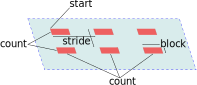
\includegraphics[scale=2.0]{selection.pdf}
\label{fig:hyperslab}
\caption{hyper-slab illustration}
\end{figure}
   
\subsection{Transformation}

\subsection{Writing}

\subsection{Update}

\subsection{Extension}

\subsection{Poststructure}



\section{Datatest with GoogleTest Framework}
\subsection{Initialization}
\subsection{Testfissure}
\subsection{Testclass including HDF5 Interface}


%\nocite{*}


\bibliographystyle{plain}
\bibliography{references,wp,own}

\end{document}
